\documentclass[12pt]{article}
\usepackage[utf8]{inputenc}
\usepackage[english, russian]{babel}
\usepackage{graphicx, float, multicol, hyperref, pgfplots}

\title{Определение модуля Юнга на основе исследования деформаций растяжения и изгиба}
\author{Балдин Виктор}

\begin{document}
    \maketitle

    \section{Aннотация}
    \textbf{Цель работы:} экспериментально получить зависимость между напряжением и деформацией
    для двух простейших напряженных состояний упругих тел: одностороннего сжатия и чистого изгиба;
    по результатам эксперимента вычислить модул Юнга.\\
    \textbf{В работе используются:} в первой части - прибор Лермантова, проволка
    из исследуемого материала,
     зрительная трубка со шкалой,
    набор грузов, микрометр,рулетка;  во второй части - стойка для изгибания балки, индикатор для
    измерения величин прогиба,
набор исследуемых стержней, грузы, линейка, штангенциркуль.

    \section{Теоретические сведения}
    Растяжение проволки соответствует напряженому состоянию вдоль одной оси, которое описывается формулой:
\begin{equation}
    \frac{F}{S} = E \frac{\Delta l}{l}
    \label{lermantov}
\end{equation}
Измерения производятся на установке Лермантова.
Направим зрительную трубку на зеркальце.
Тогда учитывая параксиальность углов,
для расчета растяжения проволки справедлива формула:
\begin{equation}
    l = n\frac{r}{2h},
    \label{dlina}
\end{equation}
где $h$ - расстояние от шкалы до зеркальца,
$r$ - длина рычага, n - показания шкалы\\

    \section{Методика измерений}
    \begin{figure}[H]
        \centering
        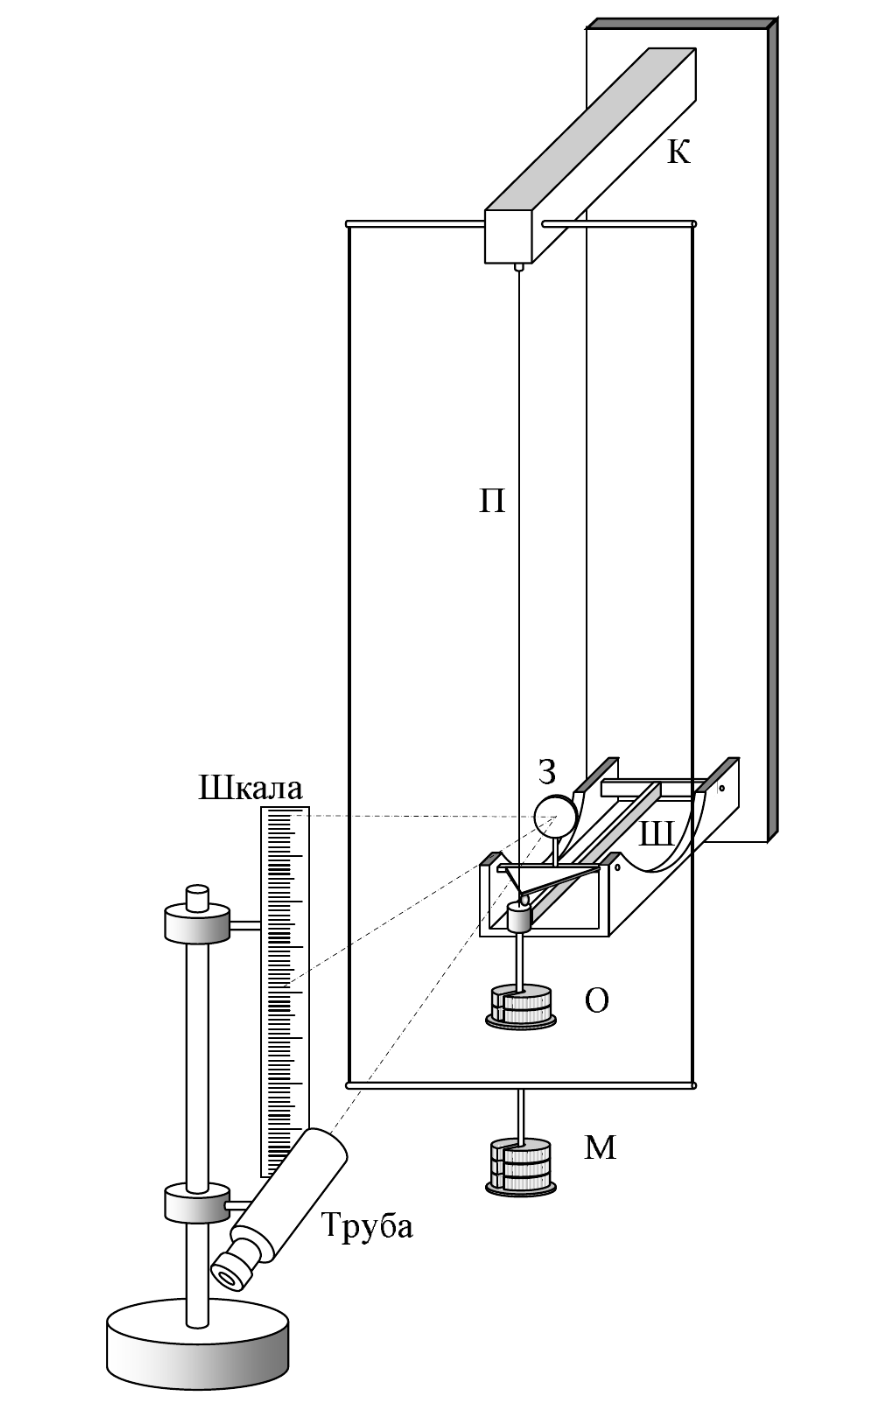
\includegraphics[scale = 0.35]{pictures/lermantov.png}
        \caption{Прибор Лермантова}
    \end{figure}

\end{document}
